\section{EO$<$ F $>$ Class Template Reference}
\label{class_e_o}\index{EO@{EO}}
EO is a base class for evolvable objects, that is, the subjects of evolution.  


{\tt \#include $<$EO.h$>$}

Inheritance diagram for EO$<$ F $>$::\begin{figure}[H]
\begin{center}
\leavevmode
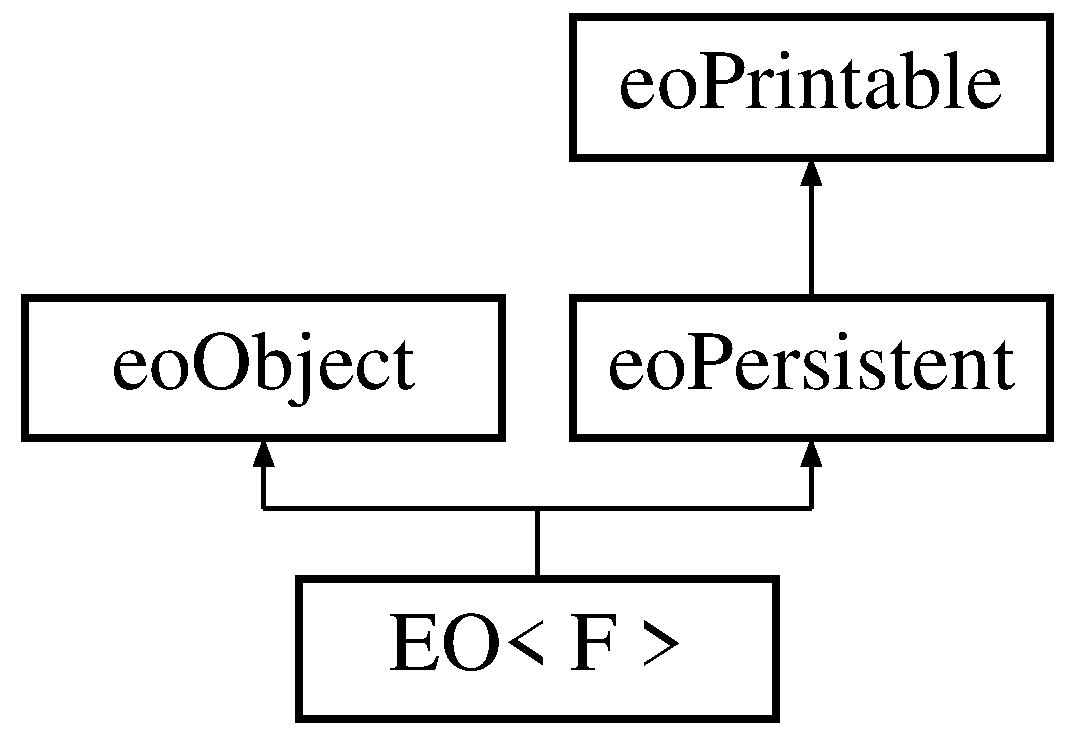
\includegraphics[height=3cm]{class_e_o}
\end{center}
\end{figure}
\subsection*{Public Types}
\begin{CompactItemize}
\item 
typedef F {\bf Fitness}\label{class_e_o_w0}

\item 
typedef Traits {\bf fitness\_\-traits}\label{class_e_o_w1}

\item 
typedef Traits::storage\_\-type {\bf storage\_\-type}\label{class_e_o_w2}

\item 
typedef Traits::performance\_\-type {\bf performance\_\-type}\label{class_e_o_w3}

\item 
typedef Traits::worth\_\-type {\bf worth\_\-type}\label{class_e_o_w4}

\end{CompactItemize}
\subsection*{Public Member Functions}
\begin{CompactItemize}
\item 
{\bf EO} ()
\begin{CompactList}\small\item\em Default constructor. \item\end{CompactList}\item 
virtual {\bf $\sim$EO} ()\label{class_e_o_a1}

\begin{CompactList}\small\item\em Virtual dtor. \item\end{CompactList}\item 
Fitness {\bf fitness} () const \label{class_e_o_a2}

\begin{CompactList}\small\item\em Return fitness value. \item\end{CompactList}\item 
void {\bf invalidate} ()\label{class_e_o_a3}

\item 
void {\bf fitness} (const Fitness \&\_\-fitness)
\begin{CompactList}\small\item\em Set fitness. \item\end{CompactList}\item 
bool {\bf invalid} () const 
\begin{CompactList}\small\item\em Return true If fitness value is invalid, false otherwise. \item\end{CompactList}\item 
bool {\bf operator$<$} (const {\bf EO} \&\_\-eo2) const 
\begin{CompactList}\small\item\em Returns true if. \item\end{CompactList}\item 
bool {\bf operator$>$} (const {\bf EO} \&\_\-eo2) const \label{class_e_o_a7}

\item 
void {\bf fitness} (performance\_\-type perf)\label{class_e_o_a9}

\item 
void {\bf performance} (performance\_\-type perf)\label{class_e_o_a10}

\item 
performance\_\-type {\bf performance} (void) const \label{class_e_o_a11}

\item 
void {\bf worth} (worth\_\-type worth)\label{class_e_o_a12}

\item 
worth\_\-type {\bf worth} (void) const \label{class_e_o_a13}

\item 
worth\_\-type {\bf fitness} (void) const \label{class_e_o_a14}

\item 
void {\bf invalidate} (void)\label{class_e_o_a15}

\item 
void {\bf invalidate\_\-worth} (void)\label{class_e_o_a16}

\item 
bool {\bf operator$<$} (const EO$<$ Fitness, Traits $>$ \&other) const \label{class_e_o_a17}

\item 
bool {\bf operator$>$} (const EO$<$ Fitness, Traits $>$ \&other) const \label{class_e_o_a18}

\end{CompactItemize}
{\bf }\par
\begin{CompactItemize}
\item 
virtual std::string {\bf class\-Name} () const 
\begin{CompactList}\small\item\em Return the class id. \item\end{CompactList}\item 
virtual void {\bf read\-From} (std::istream \&\_\-is)
\begin{CompactList}\small\item\em Read object.$\backslash$ Calls base class, just in case that one had something to do. \item\end{CompactList}\item 
virtual void {\bf print\-On} (std::ostream \&\_\-os) const 
\begin{CompactList}\small\item\em Write object. \item\end{CompactList}\end{CompactItemize}

\subsection*{Private Attributes}
\begin{CompactItemize}
\item 
Fitness {\bf rep\-Fitness}\label{class_e_o_r0}

\item 
bool {\bf invalid\-Fitness}\label{class_e_o_r1}

\item 
bool {\bf valid\_\-performance}\label{class_e_o_r2}

\item 
bool {\bf valid\_\-worth}\label{class_e_o_r3}

\item 
storage\_\-type {\bf rep\_\-fitness}\label{class_e_o_r4}

\end{CompactItemize}


\subsection{Detailed Description}
\subsubsection*{template$<$class F$>$ class EO$<$ F $>$}

EO is a base class for evolvable objects, that is, the subjects of evolution. 

EOs have only got a fitness, which at the same time needs to be only an object with the operation less than ($<$) defined. Fitness says how good is the object; evolution or change of these objects is left to the genetic operators. A fitness less than another means a worse fitness, in whatever the context; thus, fitness is always maximized; although it can be minimized with a proper definition of the $<$ operator. The fitness object must have, besides an void ctor, a copy ctor. 



Definition at line 44 of file EO.h.

\subsection{Constructor \& Destructor Documentation}
\index{EO@{EO}!EO@{EO}}
\index{EO@{EO}!EO@{EO}}
\subsubsection{\setlength{\rightskip}{0pt plus 5cm}template$<$class F$>$ {\bf EO}$<$ F $>$::{\bf EO} ()\hspace{0.3cm}{\tt  [inline]}}\label{class_e_o_a0}


Default constructor. 

Fitness must have a ctor which takes 0 as a value; we can not use void ctors here since default types like float have no void initializer. VC++ allows it, but gcc does not 

Definition at line 54 of file EO.h.

\subsection{Member Function Documentation}
\index{EO@{EO}!fitness@{fitness}}
\index{fitness@{fitness}!EO@{EO}}
\subsubsection{\setlength{\rightskip}{0pt plus 5cm}template$<$class F$>$ void {\bf EO}$<$ F $>$::fitness (const Fitness \& {\em \_\-fitness})\hspace{0.3cm}{\tt  [inline]}}\label{class_e_o_a4}


Set fitness. 

At the same time, validates it. \begin{Desc}
\item[Parameters:]
\begin{description}
\item[{\em \_\-fitness}]New fitness value. \end{description}
\end{Desc}


Definition at line 72 of file EO.h.\index{EO@{EO}!invalid@{invalid}}
\index{invalid@{invalid}!EO@{EO}}
\subsubsection{\setlength{\rightskip}{0pt plus 5cm}template$<$class F$>$ bool {\bf EO}$<$ F $>$::invalid () const\hspace{0.3cm}{\tt  [inline]}}\label{class_e_o_a5}


Return true If fitness value is invalid, false otherwise. 

\begin{Desc}
\item[Returns:]true If fitness is invalid. \end{Desc}


Definition at line 81 of file EO.h.

Referenced by EO$<$ Py\-Fitness $>$::fitness(), eo\-One\-Max\-Eval\-Func$<$ EOT $>$::operator()(), eo\-One\-Fifth\-Mutation$<$ EOT $>$::operator()(), eo\-Eval\-Func\-Ptr$<$ EOT, Fit\-T, Function\-Arg $>$::operator()(), eo\-Eval\-Func\-Counter$<$ EOT $>$::operator()(), and EO$<$ Py\-Fitness $>$::print\-On().\index{EO@{EO}!operator<@{operator$<$}}
\index{operator<@{operator$<$}!EO@{EO}}
\subsubsection{\setlength{\rightskip}{0pt plus 5cm}template$<$class F$>$ bool {\bf EO}$<$ F $>$::operator$<$ (const {\bf EO}$<$ F $>$ \& {\em \_\-eo2}) const\hspace{0.3cm}{\tt  [inline]}}\label{class_e_o_a6}


Returns true if. 

\begin{Desc}
\item[Returns:]true if the fitness is higher \end{Desc}


Definition at line 86 of file EO.h.

Referenced by eo\-Vector$<$ Fit\-T, bool $>$::operator$<$().\index{EO@{EO}!className@{className}}
\index{className@{className}!EO@{EO}}
\subsubsection{\setlength{\rightskip}{0pt plus 5cm}template$<$class F$>$ virtual std::string {\bf EO}$<$ F $>$::class\-Name (void) const\hspace{0.3cm}{\tt  [inline, virtual]}}\label{class_e_o_z10_0}


Return the class id. 

\begin{Desc}
\item[Returns:]the class name as a std::string \end{Desc}


Implements {\bf eo\-Object} {\rm (p.\,\pageref{classeo_object_a1})}.

Reimplemented in {\bf eo\-Es\-Full$<$ Fit $>$} {\rm (p.\,\pageref{classeo_es_full_a1})}, {\bf eo\-Es\-Simple$<$ Fit $>$} {\rm (p.\,\pageref{classeo_es_simple_a1})}, {\bf eo\-Es\-Stdev$<$ Fit $>$} {\rm (p.\,\pageref{classeo_es_stdev_a1})}, {\bf eo\-Real$<$ Fit\-T $>$} {\rm (p.\,\pageref{classeo_real_a1})}, {\bf eo\-Bit$<$ Fit\-T $>$} {\rm (p.\,\pageref{classeo_bit_a1})}, {\bf eo\-Parse\-Tree$<$ FType, Node $>$} {\rm (p.\,\pageref{classeo_parse_tree_a4})}, {\bf eo\-String$<$ fitness\-T $>$} {\rm (p.\,\pageref{classeo_string_z26_0})}, and {\bf eo\-One\-Max$<$ Fit\-T $>$} {\rm (p.\,\pageref{classeo_one_max_a2})}.

Definition at line 95 of file EO.h.\index{EO@{EO}!readFrom@{readFrom}}
\index{readFrom@{readFrom}!EO@{EO}}
\subsubsection{\setlength{\rightskip}{0pt plus 5cm}template$<$class F$>$ virtual void {\bf EO}$<$ F $>$::read\-From (std::istream \& {\em \_\-is})\hspace{0.3cm}{\tt  [inline, virtual]}}\label{class_e_o_z10_1}


Read object.$\backslash$ Calls base class, just in case that one had something to do. 

The read and print methods should be compatible and have the same format. In principle, format is \char`\"{}plain\char`\"{}: they just print a number \begin{Desc}
\item[Parameters:]
\begin{description}
\item[{\em \_\-is}]a std::istream. \end{description}
\end{Desc}
\begin{Desc}
\item[Exceptions:]
\begin{description}
\item[{\em runtime\_\-std::exception}]If a valid object can't be read. \end{description}
\end{Desc}


Implements {\bf eo\-Persistent} {\rm (p.\,\pageref{classeo_persistent_a1})}.

Reimplemented in {\bf eo\-Vector$<$ Fit\-T, Gene\-Type $>$} {\rm (p.\,\pageref{classeo_vector_a5})}, {\bf eo\-Es\-Full$<$ Fit $>$} {\rm (p.\,\pageref{classeo_es_full_a3})}, {\bf eo\-Es\-Simple$<$ Fit $>$} {\rm (p.\,\pageref{classeo_es_simple_a3})}, {\bf eo\-Es\-Stdev$<$ Fit $>$} {\rm (p.\,\pageref{classeo_es_stdev_a3})}, {\bf eo\-Bit$<$ Fit\-T $>$} {\rm (p.\,\pageref{classeo_bit_a3})}, {\bf eo\-Parse\-Tree$<$ FType, Node $>$} {\rm (p.\,\pageref{classeo_parse_tree_a6})}, {\bf eo\-External\-EO$<$ Fit, External $>$} {\rm (p.\,\pageref{classeo_external_e_o_a3})}, {\bf eo\-Vector$<$ Fit, double $>$} {\rm (p.\,\pageref{classeo_vector_a5})}, {\bf eo\-Vector$<$ Fit\-T, double $>$} {\rm (p.\,\pageref{classeo_vector_a5})}, and {\bf eo\-Vector$<$ Fit\-T, bool $>$} {\rm (p.\,\pageref{classeo_vector_a5})}.

Definition at line 105 of file EO.h.

Referenced by eo\-Vector$<$ Fit\-T, bool $>$::read\-From(), eo\-Pop$<$ Dummy $>$::read\-From(), eo\-Parse\-Tree$<$ FType, Node $>$::read\-From(), eo\-One\-Max$<$ Fit\-T $>$::read\-From(), eo\-External\-EO$<$ Fit, External $>$::read\-From(), and eo\-Bit$<$ Fit\-T $>$::read\-From().\index{EO@{EO}!printOn@{printOn}}
\index{printOn@{printOn}!EO@{EO}}
\subsubsection{\setlength{\rightskip}{0pt plus 5cm}template$<$class F$>$ virtual void {\bf EO}$<$ F $>$::print\-On (std::ostream \& {\em \_\-os}) const\hspace{0.3cm}{\tt  [inline, virtual]}}\label{class_e_o_z10_2}


Write object. 

Called print\-On since it prints the object \_\-on\_\- a stream. \begin{Desc}
\item[Parameters:]
\begin{description}
\item[{\em \_\-os}]A std::ostream. \end{description}
\end{Desc}


Implements {\bf eo\-Printable} {\rm (p.\,\pageref{classeo_printable_a1})}.

Reimplemented in {\bf eo\-Vector$<$ Fit\-T, Gene\-Type $>$} {\rm (p.\,\pageref{classeo_vector_a4})}, {\bf eo\-Es\-Full$<$ Fit $>$} {\rm (p.\,\pageref{classeo_es_full_a2})}, {\bf eo\-Es\-Simple$<$ Fit $>$} {\rm (p.\,\pageref{classeo_es_simple_a2})}, {\bf eo\-Es\-Stdev$<$ Fit $>$} {\rm (p.\,\pageref{classeo_es_stdev_a2})}, {\bf eo\-Bit$<$ Fit\-T $>$} {\rm (p.\,\pageref{classeo_bit_a2})}, {\bf eo\-Parse\-Tree$<$ FType, Node $>$} {\rm (p.\,\pageref{classeo_parse_tree_a5})}, {\bf eo\-External\-EO$<$ Fit, External $>$} {\rm (p.\,\pageref{classeo_external_e_o_a4})}, {\bf eo\-String$<$ fitness\-T $>$} {\rm (p.\,\pageref{classeo_string_z24_1})}, {\bf Dummy} {\rm (p.\,\pageref{struct_dummy_a1})}, {\bf Dummy} {\rm (p.\,\pageref{struct_dummy_a2})}, {\bf Dummy} {\rm (p.\,\pageref{struct_dummy_a3})}, {\bf Dummy} {\rm (p.\,\pageref{struct_dummy_a4})}, {\bf eo\-Vector$<$ Fit, double $>$} {\rm (p.\,\pageref{classeo_vector_a4})}, {\bf eo\-Vector$<$ Fit\-T, double $>$} {\rm (p.\,\pageref{classeo_vector_a4})}, and {\bf eo\-Vector$<$ Fit\-T, bool $>$} {\rm (p.\,\pageref{classeo_vector_a4})}.

Definition at line 129 of file EO.h.

Referenced by Dummy::print\-On(), eo\-Vector$<$ Fit\-T, bool $>$::print\-On(), eo\-String$<$ fitness\-T $>$::print\-On(), eo\-Parse\-Tree$<$ FType, Node $>$::print\-On(), eo\-One\-Max$<$ Fit\-T $>$::print\-On(), eo\-External\-EO$<$ Fit, External $>$::print\-On(), and eo\-Bit$<$ Fit\-T $>$::print\-On().

The documentation for this class was generated from the following files:\begin{CompactItemize}
\item 
EO.h\item 
fitness\_\-traits.cpp\end{CompactItemize}
